\documentclass[11pt,a4paper]{article}
\usepackage[margin=2.6cm]{geometry}
\usepackage{amsmath,amssymb}
\usepackage{booktabs}
\usepackage{xcolor}
\usepackage{tikz}
\usetikzlibrary{arrows.meta,positioning,fit,backgrounds,calc}
\usepackage[colorlinks=true,linkcolor=blue!50!black,urlcolor=blue!50!black]{hyperref}

\title{Branch and price for the 3D-SCPTOP\\
\large and what ``optimal'' does and does not mean in our results}
\author{}
\date{31 August 2026}

\newcommand{\lb}{\underline{z}}
\newcommand{\ub}{\overline{z}}

\begin{document}
\maketitle

\begin{abstract}
\noindent
This note explains the branch-and-price method as implemented, and states
precisely what our results guarantee. The short answer to the second question:
\textbf{we do not in general prove optimality, and we should not claim to}. What
we do guarantee is different and, for this problem, arguably more valuable ---
\textbf{every truck we report is proven loadable}. The distinction matters
because the software once reported a solution as \texttt{OPTIMAL} that its own
lower bound admitted could be $24\%$ above optimal.
\end{abstract}

\section{Why decompose at all}

The compact 3D-SCPTOP carries a variable for every combination of truck,
loading configuration, product and period. Two consequences follow. It is
enormous --- $68\,904$ variables on a four-product, ten-period instance --- and
it is \emph{symmetric}: trucks are interchangeable, so the branch-and-bound tree
explores permutations of the same plan. On the ten-period instances Gurobi
returns no feasible solution at all within half an hour.

Dantzig--Wolfe decomposition moves the geometry out of the model and into the
\emph{columns}. A column is one truck's load: a specific set of returnable
transport items, placed in specific slots, that we have already checked can
physically be built. The master problem then never reasons about packing. It
only chooses \emph{how many of each load to dispatch, and when}.

\begin{center}
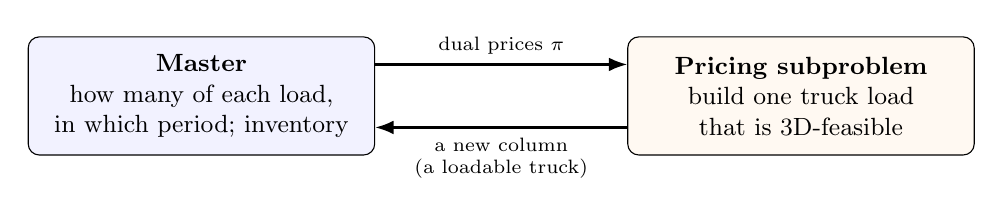
\begin{tikzpicture}[font=\small,node distance=6mm]
  \node[draw,rounded corners,fill=blue!5,minimum width=4.4cm,minimum height=1.5cm,align=center]
    (m) {\textbf{Master}\\ how many of each load,\\ in which period; inventory};
  \node[draw,rounded corners,fill=orange!5,minimum width=4.4cm,minimum height=1.5cm,align=center,right=3.2cm of m]
    (p) {\textbf{Pricing subproblem}\\ build one truck load\\ that is 3D-feasible};
  \draw[-Latex,thick] ([yshift=4mm]m.east) -- node[above,align=center,font=\scriptsize]
    {dual prices $\pi$} ([yshift=4mm]p.west);
  \draw[-Latex,thick] ([yshift=-4mm]p.west) -- node[below,align=center,font=\scriptsize]
    {a new column\\ (a loadable truck)} ([yshift=-4mm]m.east);
\end{tikzpicture}
\end{center}

\section{The two problems}

\paragraph{Master (restricted).}
Let $\Omega$ be the set of all geometrically feasible truck loads --- far too
many to enumerate --- and $\Omega' \subset \Omega$ the ones we have generated so
far. For a load $k$, $a_{ck}$ is how many units of commodity $c$ it carries, and
$c_K$ is the cost of dispatching a truck. With $y_{kt} \geq 0$ the number of
copies of load $k$ dispatched in period $t$, and $I$ the inventory variables:
\[
\min \; c_K \sum_{k \in \Omega'} \sum_t y_{kt} \;+\; \text{(inventory cost)}
\qquad \text{s.t.} \quad
\sum_{k \in \Omega'} a_{ck}\, y_{kt} \;+\; \text{(flow, stock)} \;\geq\; d_{ct}
\]
This is a linear program. Solving it gives an objective value $z_{\mathrm{RMP}}$
and dual prices $\pi_{ct}$ on the demand rows.

\paragraph{Pricing.}
The duals say what a unit of each commodity is worth. We then ask: \emph{is
there a loadable truck worth more than it costs?} That is a 3D packing problem
solved with CP-SAT, subject to every physical rule --- slot placement, stack
crush limits, trailer payload, and the full-truckload rule (a truck must be full
\emph{by volume or by weight}, not by their sum):
\[
\max_{a \in \Omega} \; \sum_c \pi_c\, a_c
\qquad\Longrightarrow\qquad
\text{reduced cost} \;=\; c_K - \sum_c \pi_c\, a_c .
\]
If the reduced cost is negative, that load improves the master, and we add it
and re-solve. If \emph{no} load has negative reduced cost, the restricted master
is optimal for the \emph{full} problem $\Omega$ --- and this is the only
circumstance under which we learn anything certain.

\paragraph{One implementation detail that is not cosmetic.}
Dual prices are scaled to integers for CP-SAT and \textbf{rounded up, never to
nearest}. Rounding to nearest can make the oracle believe a column is unprofitable
when it is not, which destroys the proof in the next section; convergence would
then never be declared.

\section{Bounds: the part that decides whether we may say ``optimal''}

This is where the reasoning is easy to get wrong, and where we got it wrong.

\begin{quote}
\textbf{The restricted master's LP value is not a lower bound.}
$z_{\mathrm{RMP}}$ is computed over a \emph{subset} of columns. Adding columns
can only lower it. It is therefore an \emph{upper} bound on the true master LP
value $z_{\mathrm{LP}}$.
\end{quote}

Three situations, and what each licenses us to say:

\begin{center}\small
\begin{tabular}{@{}p{4.5cm}p{5.3cm}p{3.3cm}@{}}
\toprule
Situation & What is known & May we quote a gap? \\
\midrule
Pricing proved no improving column & $z_{\mathrm{RMP}} = z_{\mathrm{LP}}$, a valid lower bound & yes, a \emph{certified} gap \\
Pricing ran but did not close & Lagrangian bound applies & yes, a weaker valid gap \\
Pricing never ran (deadline) & nothing from below & \textbf{no} \\
\bottomrule
\end{tabular}
\end{center}

The middle case uses the Lagrangian (Farley) correction: if $\rho$ is the most
negative reduced cost found and $\kappa$ an upper bound on how many columns an
optimal solution can use, then
$z_{\mathrm{LP}} \geq z_{\mathrm{RMP}} + \kappa\rho$.
It is valid but loose --- across our benchmark it averages a $28.6\%$ gap, which
describes the bound, not the plans.

\begin{center}
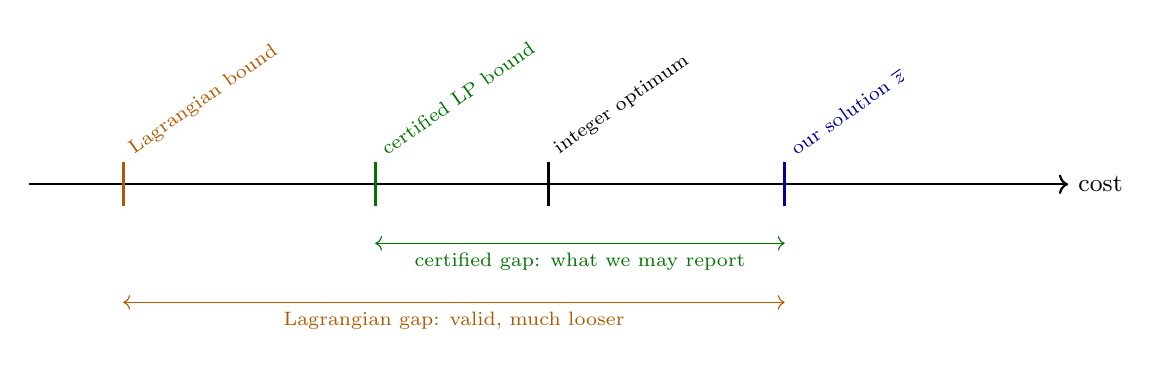
\begin{tikzpicture}[font=\small]
  \draw[->,thick] (0,0) -- (13.2,0) node[right] {cost};
  \foreach \x/\lab/\col in {1.2/{Lagrangian bound}/orange!70!black,
                            4.4/{certified LP bound}/green!45!black,
                            6.6/{integer optimum}/black,
                            9.6/{our solution $\ub$}/blue!60!black}{
     \draw[\col,very thick] (\x,-0.28) -- (\x,0.28);
     \node[\col,rotate=35,anchor=west,font=\scriptsize] at (\x,0.36) {\lab};
  }
  \draw[<->,green!45!black] (4.4,-0.75) -- node[below,font=\scriptsize]
      {certified gap: what we may report} (9.6,-0.75);
  \draw[<->,orange!70!black] (1.2,-1.5) -- node[below,font=\scriptsize]
      {Lagrangian gap: valid, much looser} (9.6,-1.5);
\end{tikzpicture}
\end{center}

\section{From fractional to integer}

Column generation solves the \emph{linear relaxation}. Integrality still has to
be recovered, and here is the honest limitation of our method: we use
\textbf{depth-first diving}, a heuristic. We repeatedly fix the most fractional
variable and re-solve, and we do not explore the alternative branch. A full
branch-and-price would; ours does not.

\begin{center}
\begin{tikzpicture}[font=\scriptsize,level distance=9mm,
    every node/.style={draw,circle,inner sep=1.4pt,fill=blue!10}]
  \node (r) {}
    child {node (a) {}
      child {node (b) {}
        child {node (c) {\phantom{x}}}
        child[missing]}
      child[missing]}
    child[missing];
  \node[draw=none,fill=none,anchor=west,align=left] at (1.6,-0.4)
    {we follow one branch to the bottom (a ``dive'')};
  \node[draw=none,fill=none,anchor=west,align=left,gray] at (1.6,-1.6)
    {the branches we never open are why no\\ optimality proof follows from the dive};
\end{tikzpicture}
\end{center}

Consequently: \textbf{a dive can prove a solution exists, never that none is
better.} Optimality can only come from the bound, never from the dive.

\section{What our statuses actually mean}

The software previously reported the \emph{restricted master's own} solver
status. \texttt{OPTIMAL} there means ``the integer master was solved to
optimality over the columns that happened to be generated'' --- a statement
about our column pool, not about the 3D-SCPTOP. Two symptoms made this concrete:

\begin{itemize}
\item Two runs of the same instance under identical settings both reported
      \texttt{OPTIMAL}, at $4250.54$ and $4252.88$. Two genuine optima of one
      problem cannot differ; the column pools differed.
\item One stored result read \texttt{PLC:OPTIMAL} beside an objective of
      $4248.48$ and its own lower bound of $3222.88$ --- a solution that might
      be $24\%$ above optimal, labelled optimal.
\end{itemize}

Statuses now say which case holds:

\begin{center}\small
\begin{tabular}{@{}p{6.6cm}p{6.9cm}@{}}
\toprule
Status & Meaning \\
\midrule
\texttt{(proven)} & pricing closed \emph{and} the gap is zero: genuinely optimal \\
\texttt{(pool; gap<=X\% vs certified bound)} & within $X\%$ of a bound pricing proved \\
\texttt{(pool; gap<=X\% vs Lagrangian bound)} & within $X\%$ of a valid but weaker bound \\
\texttt{(pool; no valid bound)} & a feasible plan; \textbf{nothing known from below} \\
\bottomrule
\end{tabular}
\end{center}

\section{The guarantee we \emph{do} make}

Optimality is the weaker claim here. The stronger one, and the point of the
paper, is \textbf{feasibility}:

\begin{quote}
Every truck in every reported plan is re-verified independently of the model
that produced it --- payload, the full-truckload floor, per-RTI-type slot
capacity, and stack crush limits.
\end{quote}

This is not ceremony. The verifier caught three distinct classes of
impossible plan during development: a truck loaded to $24\,567$\,kg on a
$24\,000$\,kg trailer; a truck dispatched $1.4\%$ full, far under the
utilisation floor; and a configuration asked for $25$ slots where $24$ exist.
None of these was caught by the optimisation model, which considered each of
them perfectly feasible.

The contrast with the volumetric benchmark is the paper's central result. SCPTOP
treats a trailer as a volume, solves in \emph{under one second}, and reports
plans $13.7\%$ cheaper than ours --- of which, on the first benchmark instance,
\textbf{18 of its 20 truck loads are proven impossible to pack}. A cheaper plan
that cannot be loaded is not a cheaper plan.

\section{Where this leaves the results}

\begin{center}
\begin{tabular}{@{}lp{9.6cm}@{}}
\toprule
Claim & Status \\
\midrule
``Our plans are loadable''   & \textbf{Guaranteed}, verified truck by truck. \\
``Our plans are optimal''    & \textbf{Not claimed.} True only where a status reads \texttt{(proven)}. \\
``Within $X\%$ of optimal''  & Claimed only against a valid bound, and the bound's kind is named. \\
``Better than the compact model'' & Claimed only at \emph{equal measured wall-clock}; an earlier version of this comparison gave the matheuristic $400$\,s against Gurobi's $1800$\,s, and its conclusions were an artefact of that handicap. \\
\bottomrule
\end{tabular}
\end{center}

Empirically, certification is rare at the budgets we use: the pricing oracle
closed the subproblem on $1$ of $18$ runs. The strongest single result is the
ten-period instance where the compact model finds nothing in half an hour and
the matheuristic returns a plan with a \emph{certified} gap of $1.42\%$ --- and
there, ``certified'' carries its full meaning.

\end{document}
